
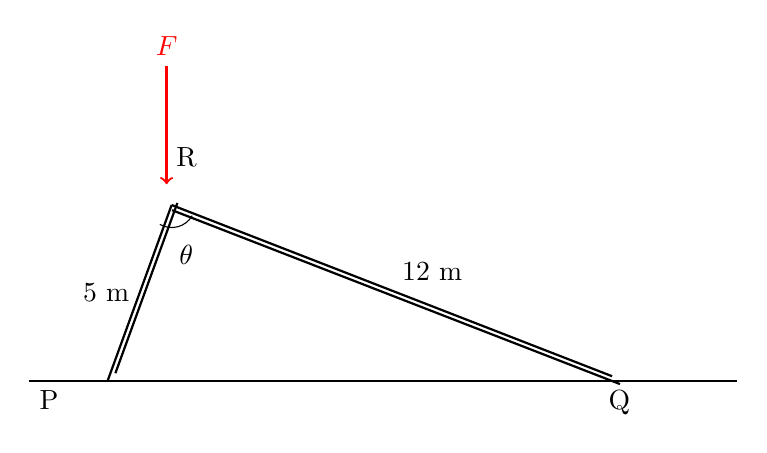
\begin{tikzpicture}
    % Draw the horizontal ground line
    \draw[thick] (-1,0) -- (8,0);

    % Draw the bar PQ (double lines)
    \draw[thick, rotate around={70:(0,0)}] (0,0) -- (2.38,0) node[midway, left] {5 m};
    \draw[thick, rotate around={70:(0.1,0.1)}] (0.1,0.1) -- (2.4,0.1);
    
    % Draw the bar QR (double lines)
    \draw[thick, rotate around={-20:(0,0)}] (0,2.38) -- (6,2.25) node[midway, above right] {12 m};
    \draw[thick, rotate around={-20:(0.1,-0.1)}] (0,2.28) -- (6.1,2.15);

    % Points P, Q, and R
    \node[below left] at (-0.5,0) {P};
    \node[below] at (6.5,0) {Q};
    \node[above right] at (0.75,2.6) {R};

    % Force arrow pointing upwards
    \draw[thick, red, <-] (0.75,2.5) -- (0.75,4) node[above] {$F$};

    % Angle theta
 \draw (1.075,2.1) arc [start angle=-30, end angle=-120, radius=0.3cm];
 \node at (1,1.6) {$\theta$};

\end{tikzpicture}

